\documentclass[11pt]{article}

\usepackage[margin=0.75in]{geometry}
\usepackage{amsfonts, amsmath, amssymb}
\usepackage[none]{hyphenat}
\usepackage{fancyhdr}
\usepackage{graphicx}
\usepackage{float}
\usepackage[nottoc, notlot, notlof]{tocbibind}

% circuitikz 
\usepackage[]{circuitikz}

\def\normalcoord(#1){coordinate(#1)}
\def\showcoord(#1){coordinate(#1) node[circle, red, draw, inner sep=1pt,
pin={[red, overlay, inner sep=0.5pt, font=\tiny, pin distance=0.1cm,
pin edge={red, overlay}]45:#1}](){}}
\let\coord=\normalcoord
\let\coord=\showcoord
% circuitikz


\pagestyle{fancy}
\fancyhead{}
\fancyfoot{}
\fancyhead[L]{Electronics (course 25032)}
\fancyhead[R]{Reza Nayeb Habib 401102694}
\fancyfoot[C]{\thepage}
\fancyfoot[R]{Sharif University of Technology}
\renewcommand{\footrulewidth}{1pt}
\parindent 0ex

\begin{document}

    
\begin{titlepage}
\begin{center}

\begin{figure}[H]
\begin{center}

\includegraphics[scale=0.4]{Fig/SUT.png}

\end{center}
\end{figure}

\huge{\textbf{Electronics 2 Projec(part 2   ) Report}} \\ 
\vspace*{2cm}
\Large{\textbf{Instructor: Dr. Medi}} \\
\vspace*{1cm}
\huge{\textbf{Sharif University of Technology}} \\
\line(1,0){500} \\ 
\Huge{\textbf{Design and Analysis of a Power Amplifier}} \\
\line(1,0){500} \\
\vfill
\Large{By Reza Nayeb Habib}\\
\Large{Student ID\# 401102694} \\

\end{center}
\end{titlepage}

\tableofcontents
\thispagestyle{empty}
\clearpage
\setcounter{page}{1}

\section{Introduction}
\section{Steps of Design and Implementation}
\section{Basic Analysis of the circuit}

\begin{figure}[H]
    \begin{center}
        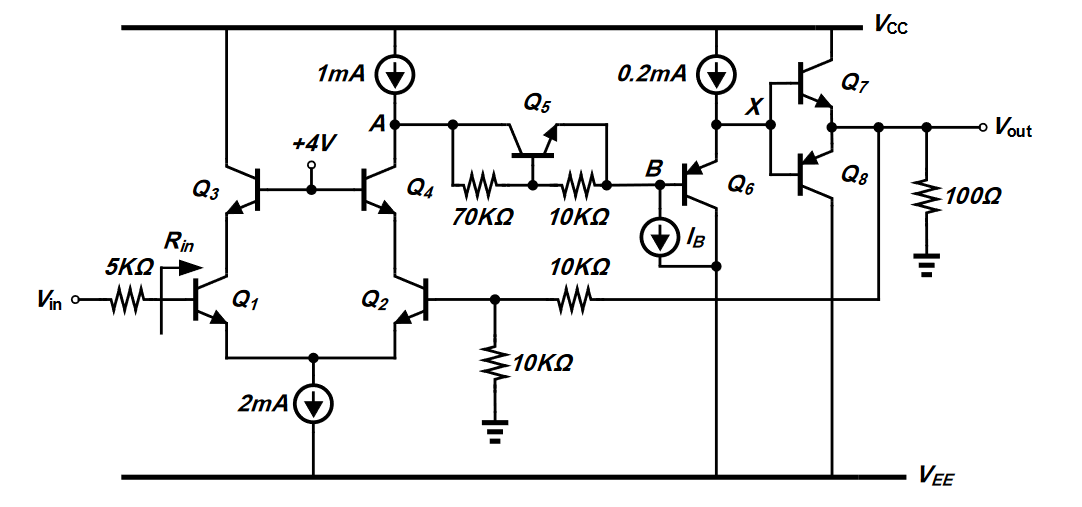
\includegraphics[scale=0.7]{Fig/circuitGiven.png}
        \label{fig:circuitGiven}
        \caption{the given circuit for the project}
    \end{center}
\end{figure}

\subsection{Finding the input and output stages}
it can be seen that the Q1, Q3 pair and Q2, Q4 pair are cascoded common emitter amplifiers
that form the differential input stage. \\
also Q7 and Q8 form a push-pull output stage.\\

\subsection{Explaining the operation of $I_B$ and Q6}
Q6 is a voltage buffer which is typically used for current gain(which we need because 
we want to design a power amplifier) and also for making the output resistance seen
be previous stages larger. \\
Q5 is a $V_{BE}$ multiplier and is used for changing the DC operating point to maximize swing.
the $V_{BE}$ multiplier only works when Q5 is on meaning the current passing from Q5
should always be positive, $I_B$ current source ensures that the current passing through Q5
is large enough and never gets negative due to the base current of Q6. \\
the maximum current of the emitter of Q6 can be 0.2mA (when all of the current source
current passes from Q6) thus the maximum of its base current is $\frac{0.2}{\beta}mA$. \\
and the current passing the Base Emitter resistor of Q5 is $ \frac{0.7}{1k} = 0.7mA $. there 
also should be a reasonable operating point current given to Q5, thus we choose
1mA to be a reasonable amount of current for the current source and choose
$I_B = 1mA$. 
\subsection{Finding the operation point of the Transistors}
for finding the operating points we can see that when $V_{in}$ is 0 then $V_{out}$ is zero
because: \\
$$ V_{in} = 0, I_{B1} \backsimeq 0 \rightarrow V_{E1} = V_{E2}  = -0.7 \rightarrow V_{B2} = 0 \rightarrow V_{out} = 0 $$
thus we can calculate the floating node voltages(like the collector nodes of transistors) by knowing the output
DC voltage. \\
here we list the operating point values(assuming $V_{BE} = 0.7V$): \\
\begin{table}[H]
    \begin{tabular}{lllllll}
    Transistor & Ic         & $V_{CE}$ \\
    Q1         & 1mA         & 4V      \\
    Q2         & 1mA         & 4V      \\
    Q3         & 1mA         & 1.6V    \\
    Q4         & 1mA         & 6.7V    \\
    Q5         & $I_B$       & 5.6V    \\
    Q6         & 0.2mA       & 10V     \\
    Q7         & 0 A         & 10V     \\
    Q8         & 0 A         & 10V     \\
    \end{tabular}
\end{table}


\subsection{Dead zone and its removal by feedback}
in type B push-pull stages due to having no bias current on zero input the transistors
will be in cutoff and will turn on when the input either reaches $V_{BE_{on}}$ or $-V_{BE_{on}}$. \\
this makes them efficient by dissipating no power at zero input and also dissipating low power on
lower inputs. the disadvantage to these stages is that until the input turns on the transistor
the output will be zero and their transfer characteristic won't be linear and they will have
some distortion(see the figure below). \\    

\begin{figure}[H]
    \begin{center}
        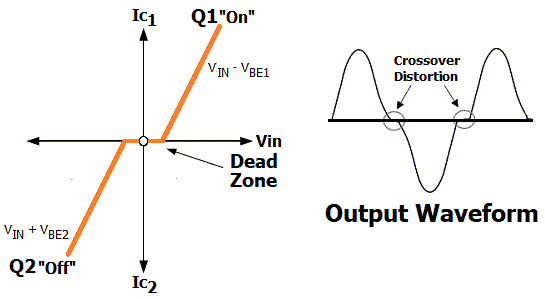
\includegraphics[scale=0.6]{Fig/deadZone.png}
        \label{fig:deadzone}
        \caption{the B class amplifier characteristic and the output distortion}
    \end{center}
\end{figure}

The problem of dead zone in push-pull amplifier can be solved (or somewhat minimized) by using
a feedback loop consider the figure below which is a simple push-pull stage with a preAmp: \\
\begin{figure}[H]
    \begin{center}
        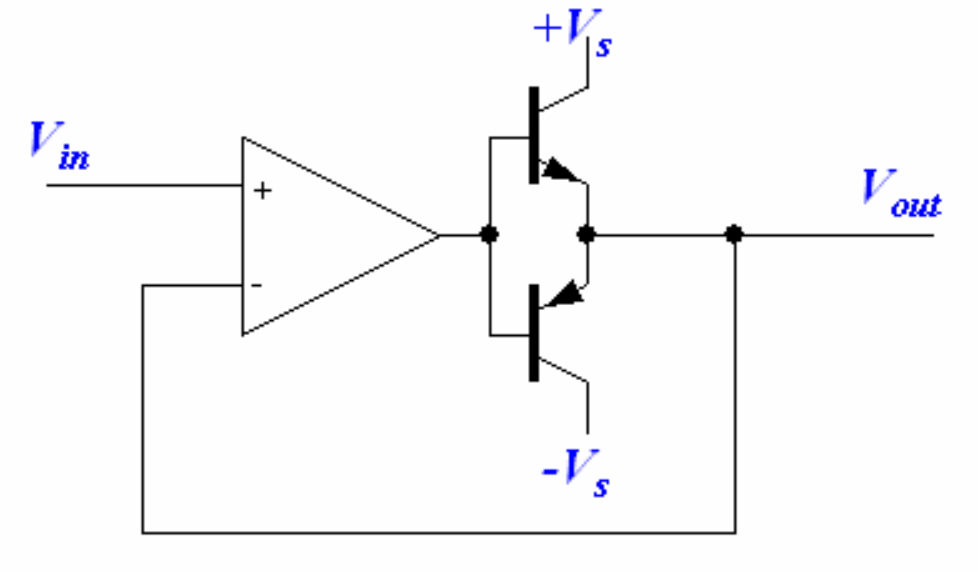
\includegraphics[scale=0.5]{Fig/preAmp.png}
        \label{fig:preAmp}
        \caption{push-pull stage with preAmp}
    \end{center}
\end{figure}

the open loop characteristic of the above circuit is that of a normal push-pull stage but with
slop of A (A is the gain of the amplifier). \\
now the loop feedback has gain $f = 1$ and the type of feedback is voltage - voltage (or series - shunt).
the closed loop gain will be $ A_v = A\frac{1}{1+Af} = \frac{A}{1+A} \backsimeq 1 $ which is the gain
we desire from a push pull stage, but the dead zone limits will now be: \\
$$ \frac{V_{BE_{on}}}{1+Af} = \frac{V_{BE_{on}}}{1+A} \backsimeq \frac{V_{BE_{on}}}{A} $$
considering that usually amplifiers have very high gain the distortion will be neglectable. \\
of course in real circuits we never put an op-amp before a push-pull stage because the push-pull
stage is part of the op-amp! but putting the stage in a feedback loop within our amplifier (as done in the
circuit of this project) will move the limits of the dead zone from $V_{BE_{on}}$ to $\frac{V_{BE_{on}}}{1+A_{OL}f}$
which again makes the dead zone size neglectable. \\

\subsection{finding ICMR and Swing}
the Input Common Mode Range (ICMR) is bounded by Q3 base voltage and the voltage needed
to be on the current source thus the common mode minimum is $ V_{EE} + V_{CS} + V_{BE_{on}}  = -9.1V $ 
and the common mode maximum is $ 4 - V_{BE_{on3}} - V_{CB_{sat1}} = 2.8V $. \\
swing analysis will be done in the next part but the result will be a swing of about
0.7V which is very low compared to the range of our voltage sources. \\

\subsection{Swing Analysis}
there are two main things in this design that prevent us from getting a high swing.
firstly node A swing is limited by the Q4 saturation voltage and node A should have 
a voltage of at least $ 4V + V_{CB_{sat}} = 4.4V $ which results in the output node swing minimum
being limited at about $ V_{out} = -0.7V $. \\
even if the above problem is solved the maximum swing would be limited by the $0.2mA$ current source.
if we assume all of the current going into the base of Q7 the output current would
be $ I_{out} = 0.2\beta mA = 30mA $ assuming $\beta = 150$. now the output voltage will
be $ V_{out} = R_{out}I_{out} = 100 \times 30mA = 3V $ which is still low
so we should either give the current source bigger current or make $\beta$ larger 
by using Darlington pair or Sziklai pair instead of the output stages NPN and PNP single transistors. \\

\subsection{the circuit schematic in LTspcie}
the schematic is shown below: \\
\begin{figure}[H]
    \begin{center}
        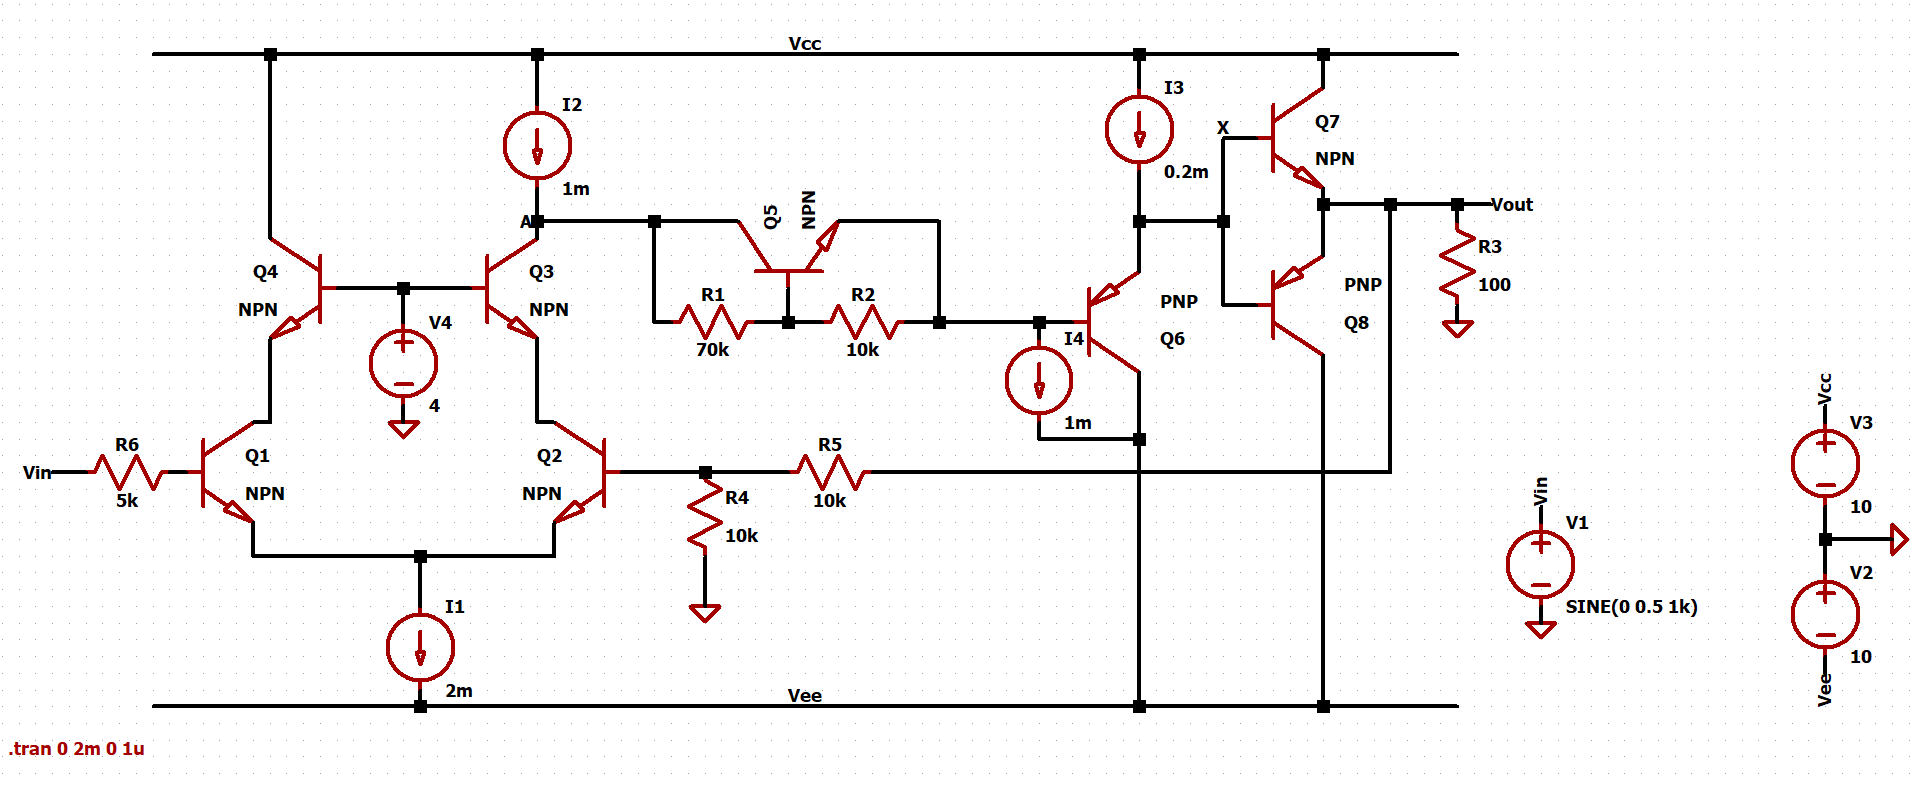
\includegraphics[scale=0.45]{Fig/circuitBasic.png}
        \label{fig:circuitBasic}
        \caption{the circuit schematic in LTspice}
    \end{center}
\end{figure}

\subsection{Voltages of the output and X node}

\begin{figure}[H]
    \begin{center}
        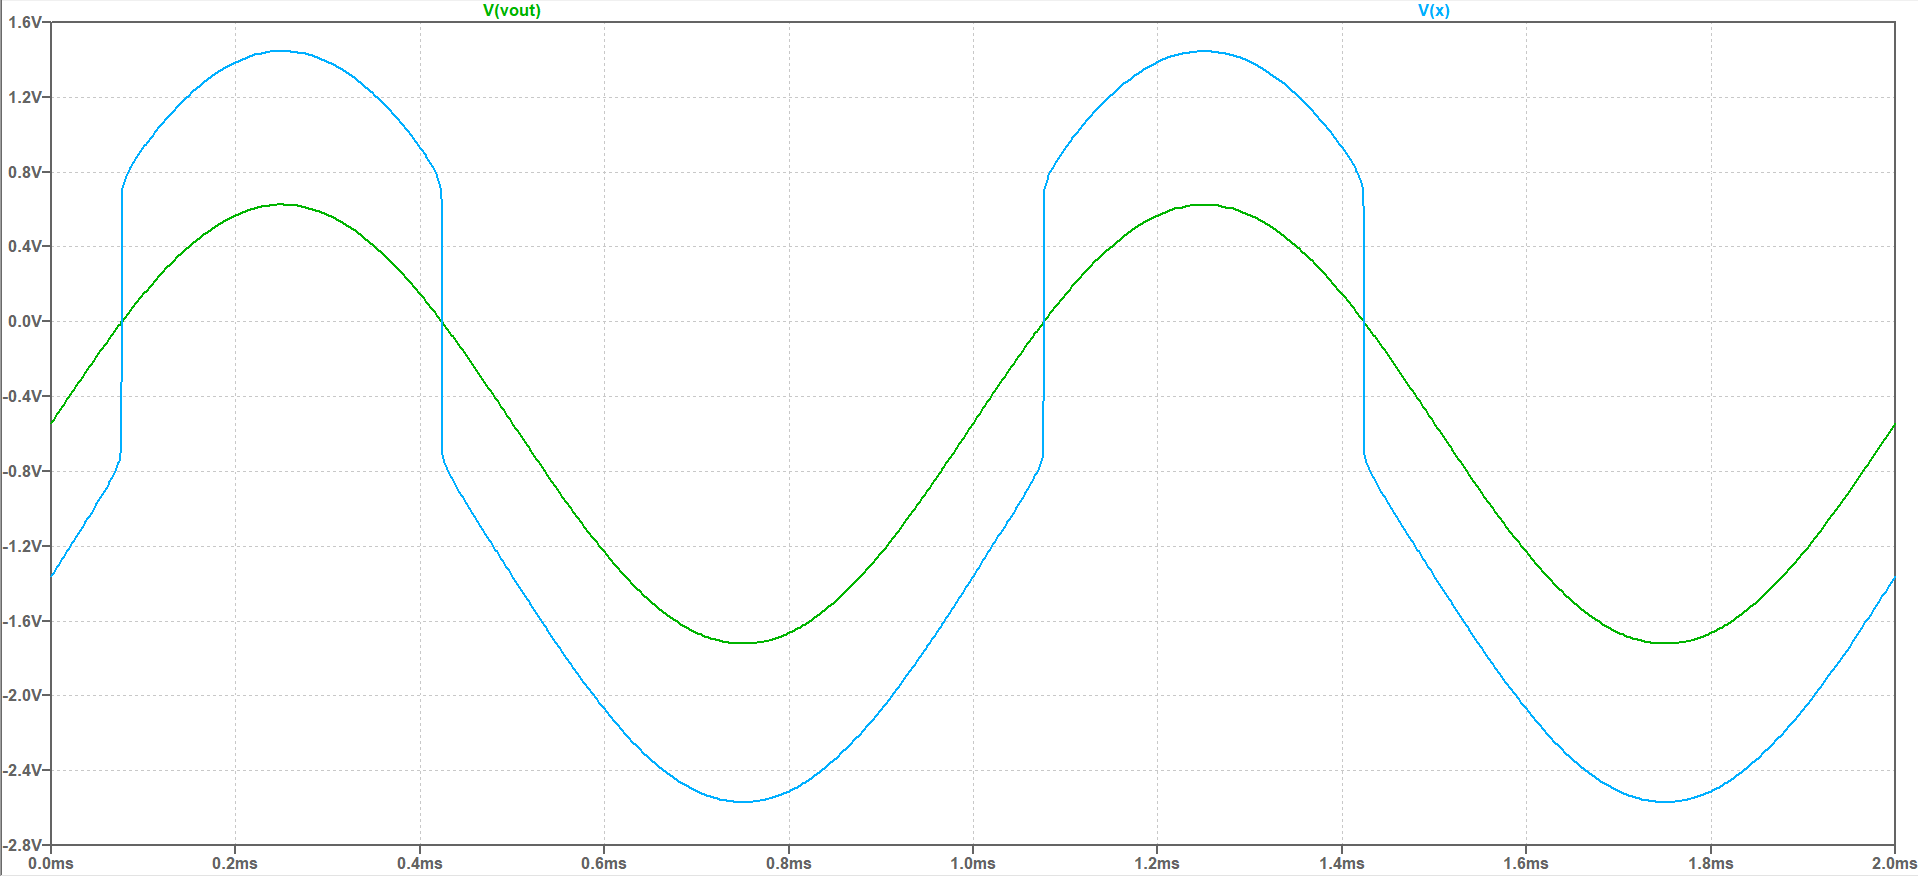
\includegraphics[scale=0.45]{Fig/outXBasic.png}
        \label{fig:outXBasic}
        \caption{the plot of output and X node in LTspice}
    \end{center}
\end{figure}

As it can be seen the dead zone that was present in the output is removed due to
feedback (just as we expected from section 4 reasoning). it is interesting that the feedback automatically handles the
dead zone problem and instead of creating a dead zone it creates sudden jumps in the voltage of
node X to smooth the output signal. \\

\subsection{Getting maximum achievable swing by changing operating points}
Removing the swing limit of the 0.2m current source is relatively easy, we will just make the current larger. \\
the real problem is the swing of node A which is limited by the 4V voltage source.
the problem is we cannot just lower the value to any number because the base of Q3 and Q4 also
limit the input voltage range and though by lowering this nodes voltage we get bigger output swing
we lose our input swing which is quite troublesome.\\
We can see that the input higher voltage limit is $ V_{source} - V_{BE_{on}} - V_{CB_{sat}} $ and the node A
lower voltage limit is $ V_{source} + V_{CB_{sat}} $ so the node should have a voltage to
handle both input and output swing. \\
by experimenting and a little tweaking we found 2V to be a reasonable value. \\
below you can see the new tweaked circuit with the maximum swing it can give: \\  

\begin{figure}[H]
    \begin{center}
        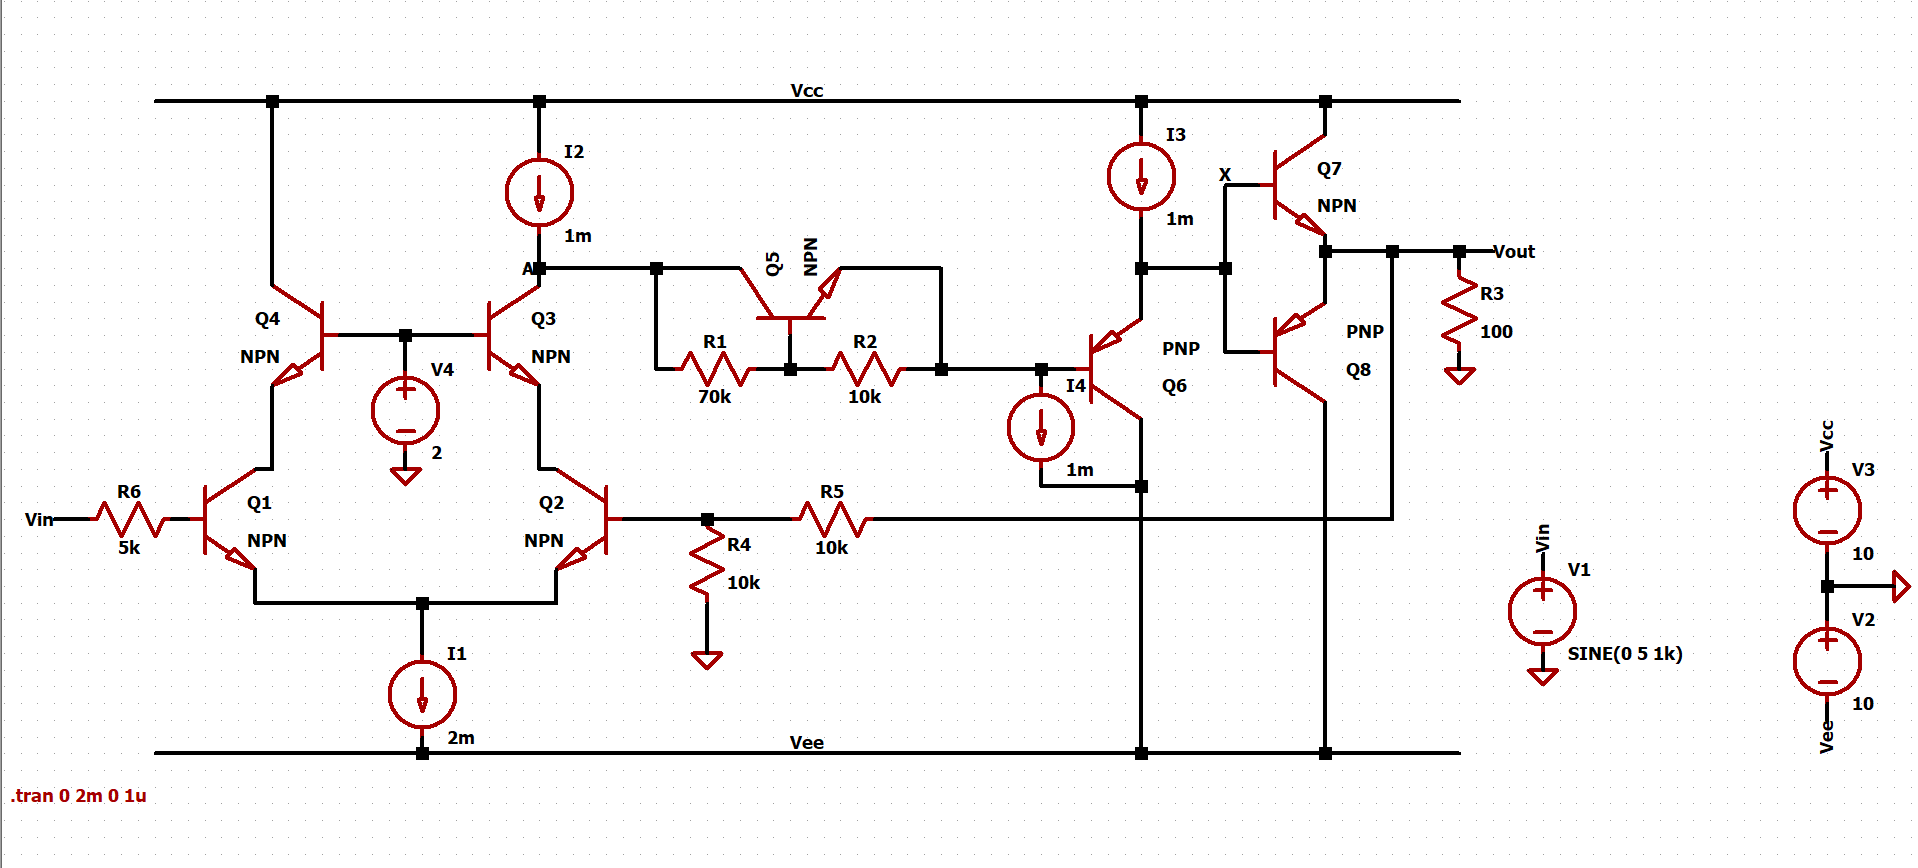
\includegraphics[scale=0.45]{Fig/circuitBasicTweaked.png}
        \label{fig:TweakedCircuit}
        \caption{the circuit with changed bias points and maximum swing in LTSPICE}
    \end{center}
\end{figure}

\begin{figure}[H]
    \begin{center}
        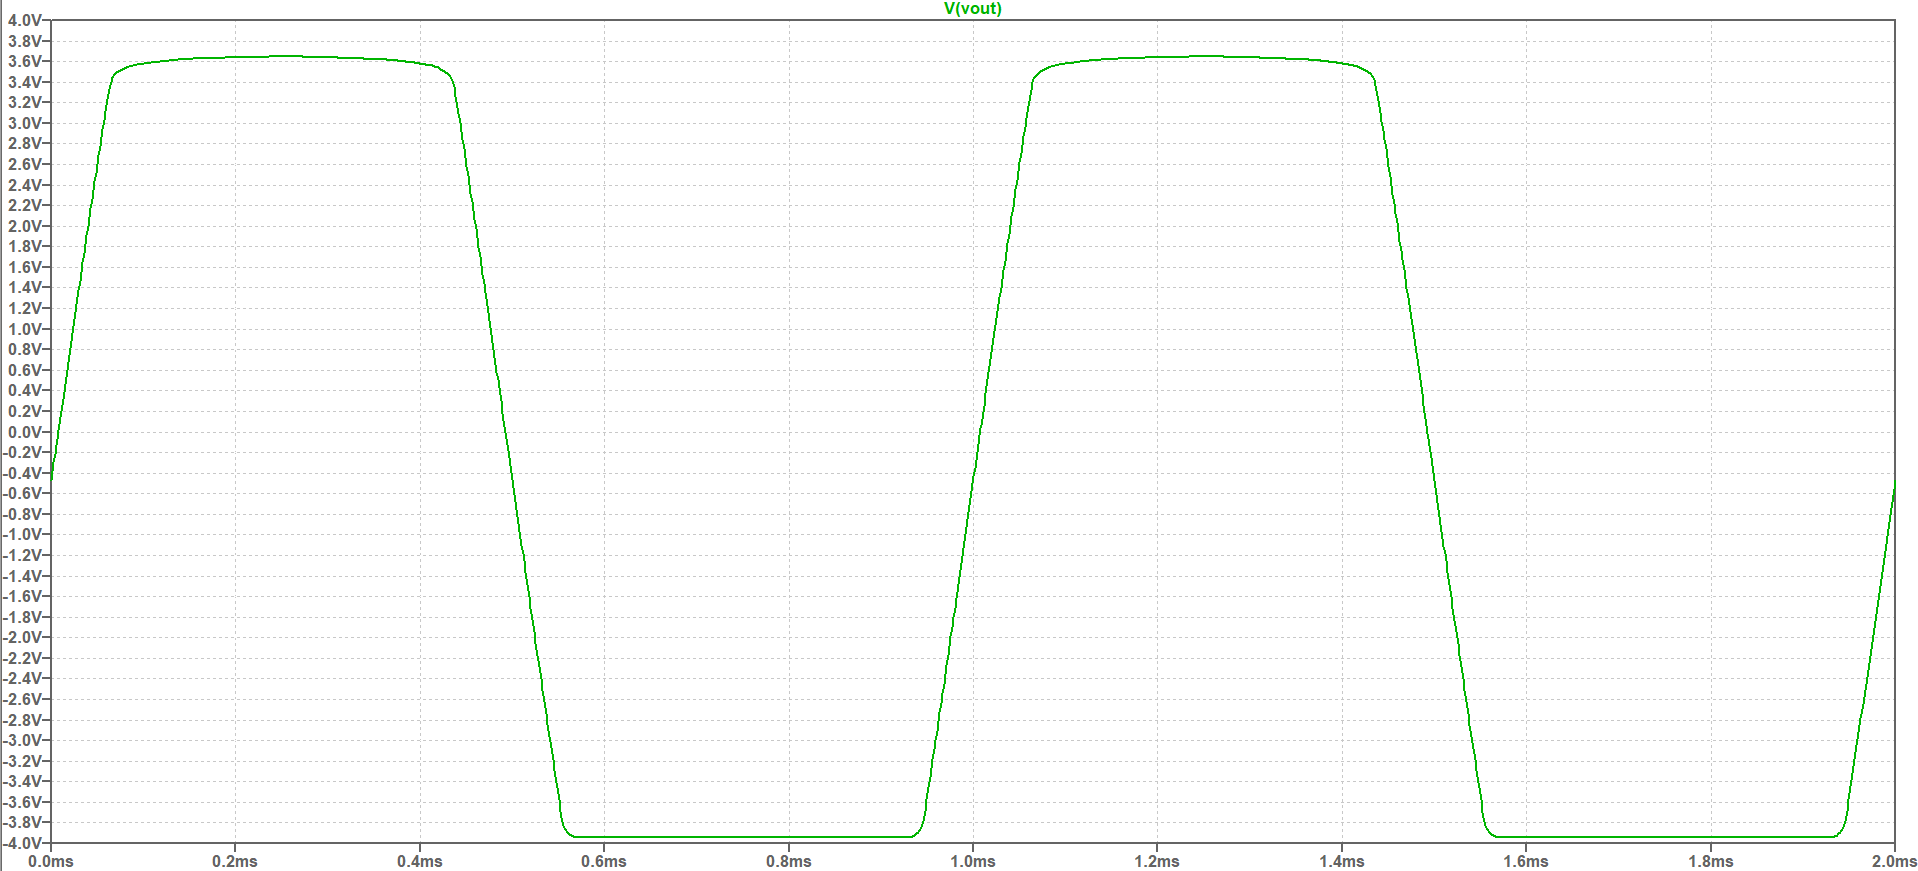
\includegraphics[scale=0.45]{Fig/outputBasicTweaked.png}
        \label{fig:TweakedOutput}
        \caption{the output with changed bias points and maximum swing in LTSPICE}
    \end{center}
\end{figure}

as it can be seen the circuit has a peak to peak swing of 7.6V or alternatively
a swing of 3.8V which is still pretty low compared to the voltage sources but better than the given
circuit. \\

\subsection{Total Harmonic Distortion (THD)}
THD or Total Harmonic Distortion is a measurement of how much a signal is distorted
by computing the value of energy in the output harmonics other than the fundamental frequency(for
example if the fundamental is 1kHz harmonics are 2kHz, 3kHz, 4kHz and ...) it is defined as: \\
$$ \text{THD} = \frac{\text{rms value of output except fundamental}}{\text{rms of fundamental}} $$

in LTspice we can add the directive " .fourier {Freq} V(out) " to get the THD in
out error log. \\

we did this with last part circuit and the result is as below: \\

\begin{figure}[H]
    \begin{center}
        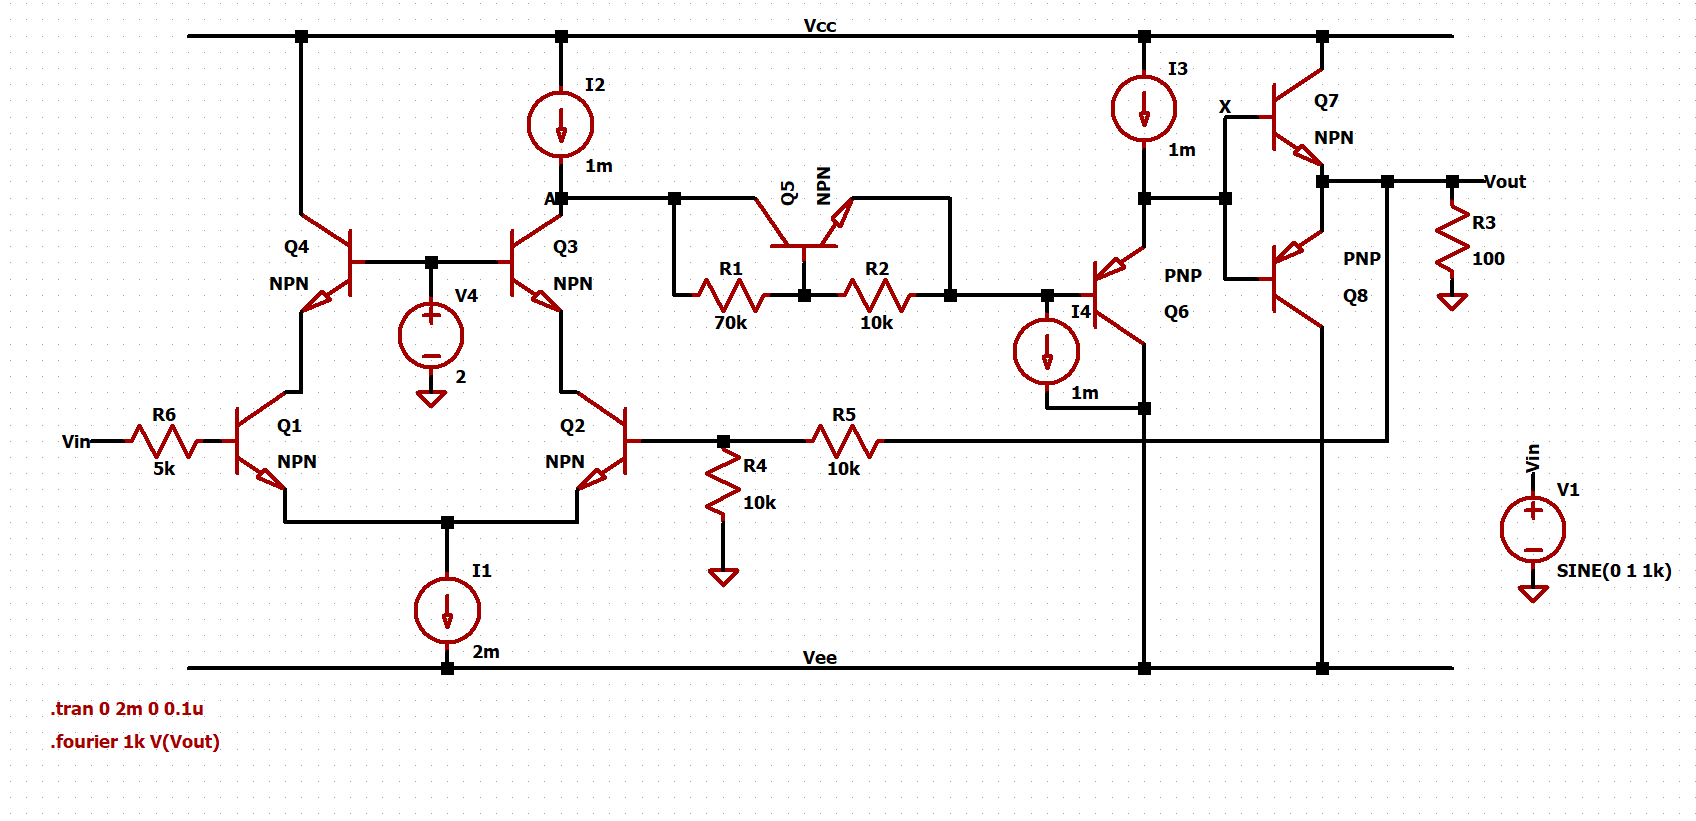
\includegraphics[scale=0.45]{Fig/circuitBasicTHD.png}
        \label{fig:TweakedCircuitTHD}
        \caption{the circuit with THD directive in LTSPICE}
    \end{center}
\end{figure}


\begin{figure}[H]
    \begin{center}
        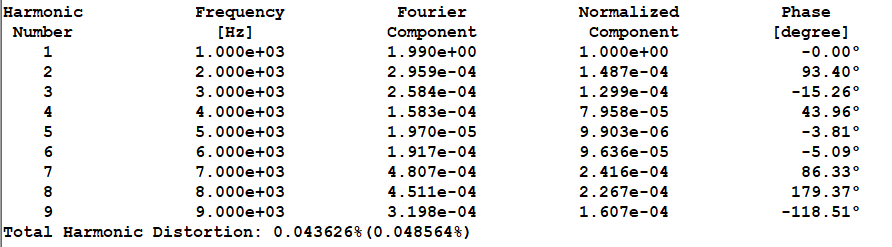
\includegraphics[scale=0.8]{Fig/THDBasic.png}
        \label{fig:THDBasic}
        \caption{THD of the circuit output in LTspice}
    \end{center}
\end{figure}
as seen above $ \text{THD} = 0.0436\% $

\section{Design}

\subsection{Folded Cascode Stage}
below you can see normal Cascode stage: \\
\begin{figure}[H]
    \begin{center}
        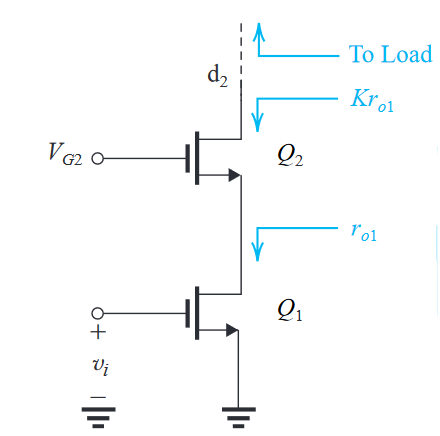
\includegraphics[scale=0.8]{Fig/cascode.png}
        \label{fig:cascode}
        \caption{Cascode Stage}
    \end{center}
\end{figure}

the problem of a normal Cascode stage is it gets a lot of headroom due to the existence of
$V_G$ (or $V_B$ in bipolar). this problem is solved in the folded Cascode stage by
making the second transistor PNP and placing it in another branch and connecting
them along with a current source, this stage does exactly the same function in small signal
but lets us swing better in large signal due to the freedom of choice for $V_G$. \\

\begin{figure}[H]
    \begin{center}
        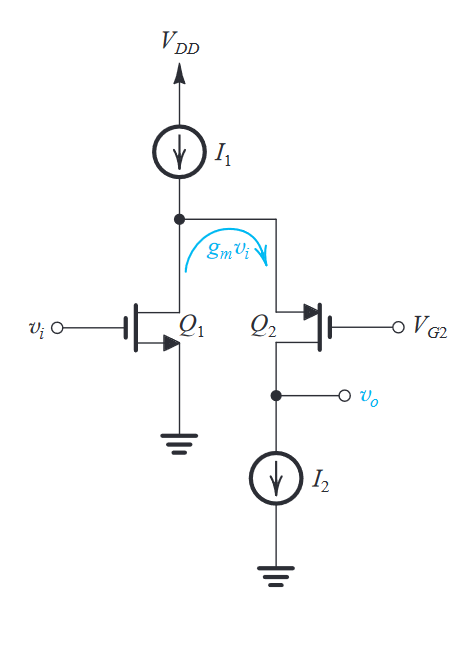
\includegraphics[scale=0.8]{Fig/folded.png}
        \label{fig:THDBasic}
        \caption{Cascode Stage}
    \end{center}
\end{figure}

also it should be noted that the folded Cascode has the disadvantage of more power usage
and the advantage that we can set $I_2$ small enough so $g_{m2}$ can get very bigger. \\


\subsection{} there are no deliverables for this section.
\subsection{Image of the Designed circuit}
\begin{figure}[H]
    \begin{center}
        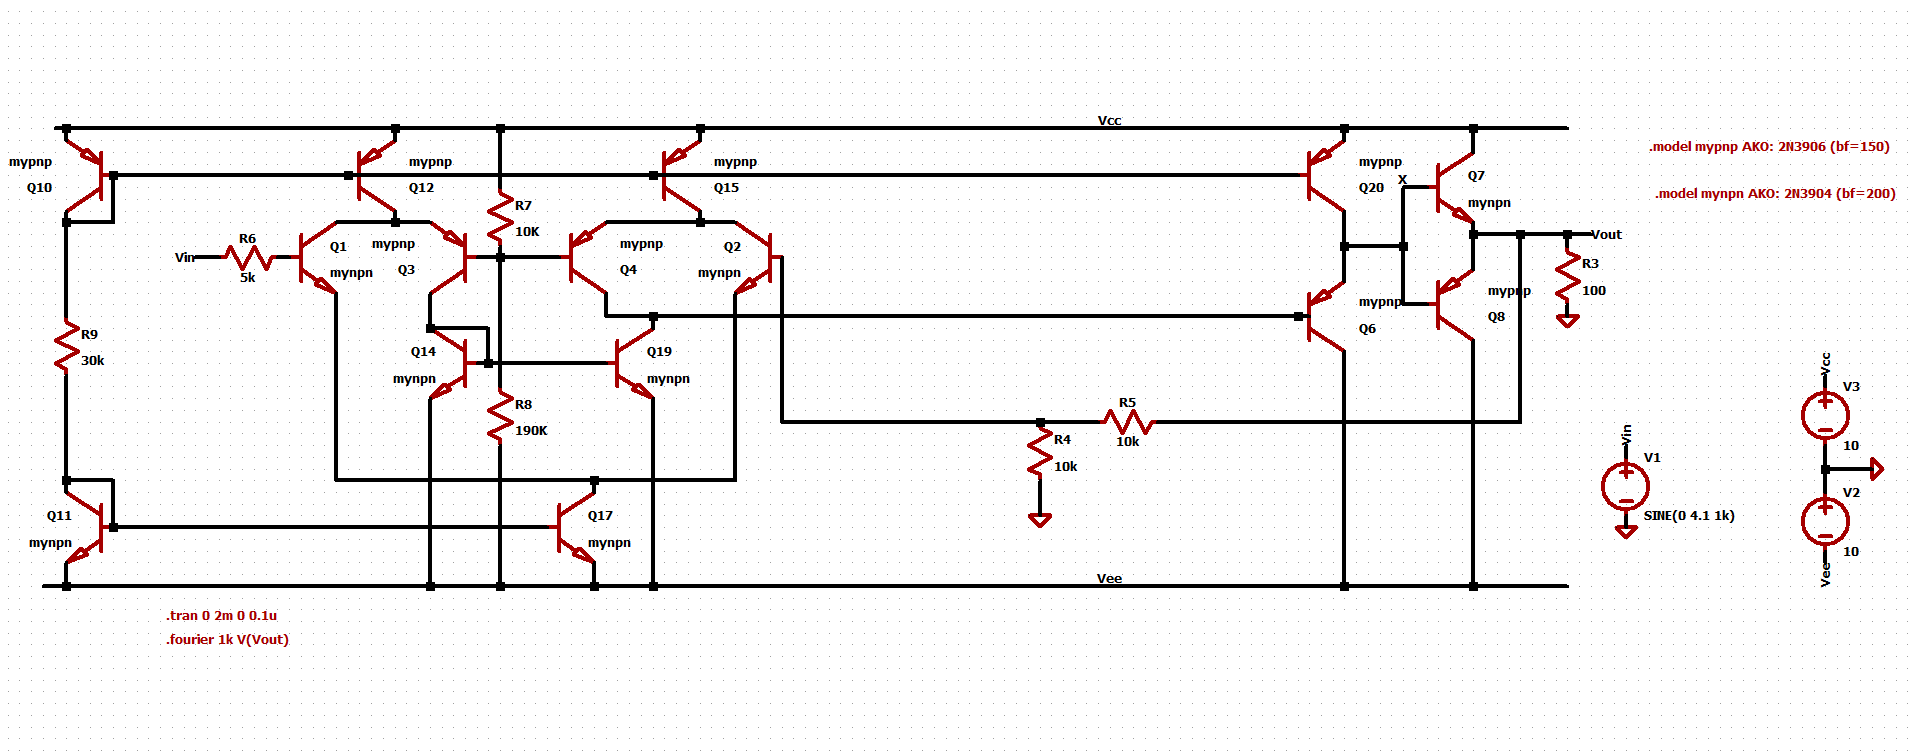
\includegraphics[scale=0.45]{Fig/circuitDesignn.png}
        \label{fig:designedCircuit}
        \caption{the Designed Circuit}
    \end{center}
\end{figure}

\subsection{}

\textbf{I. Closed Loop Gain}\\
As seen in the figure below the closed loop gain is 2: \\
\begin{figure}[H]
    \begin{center}
        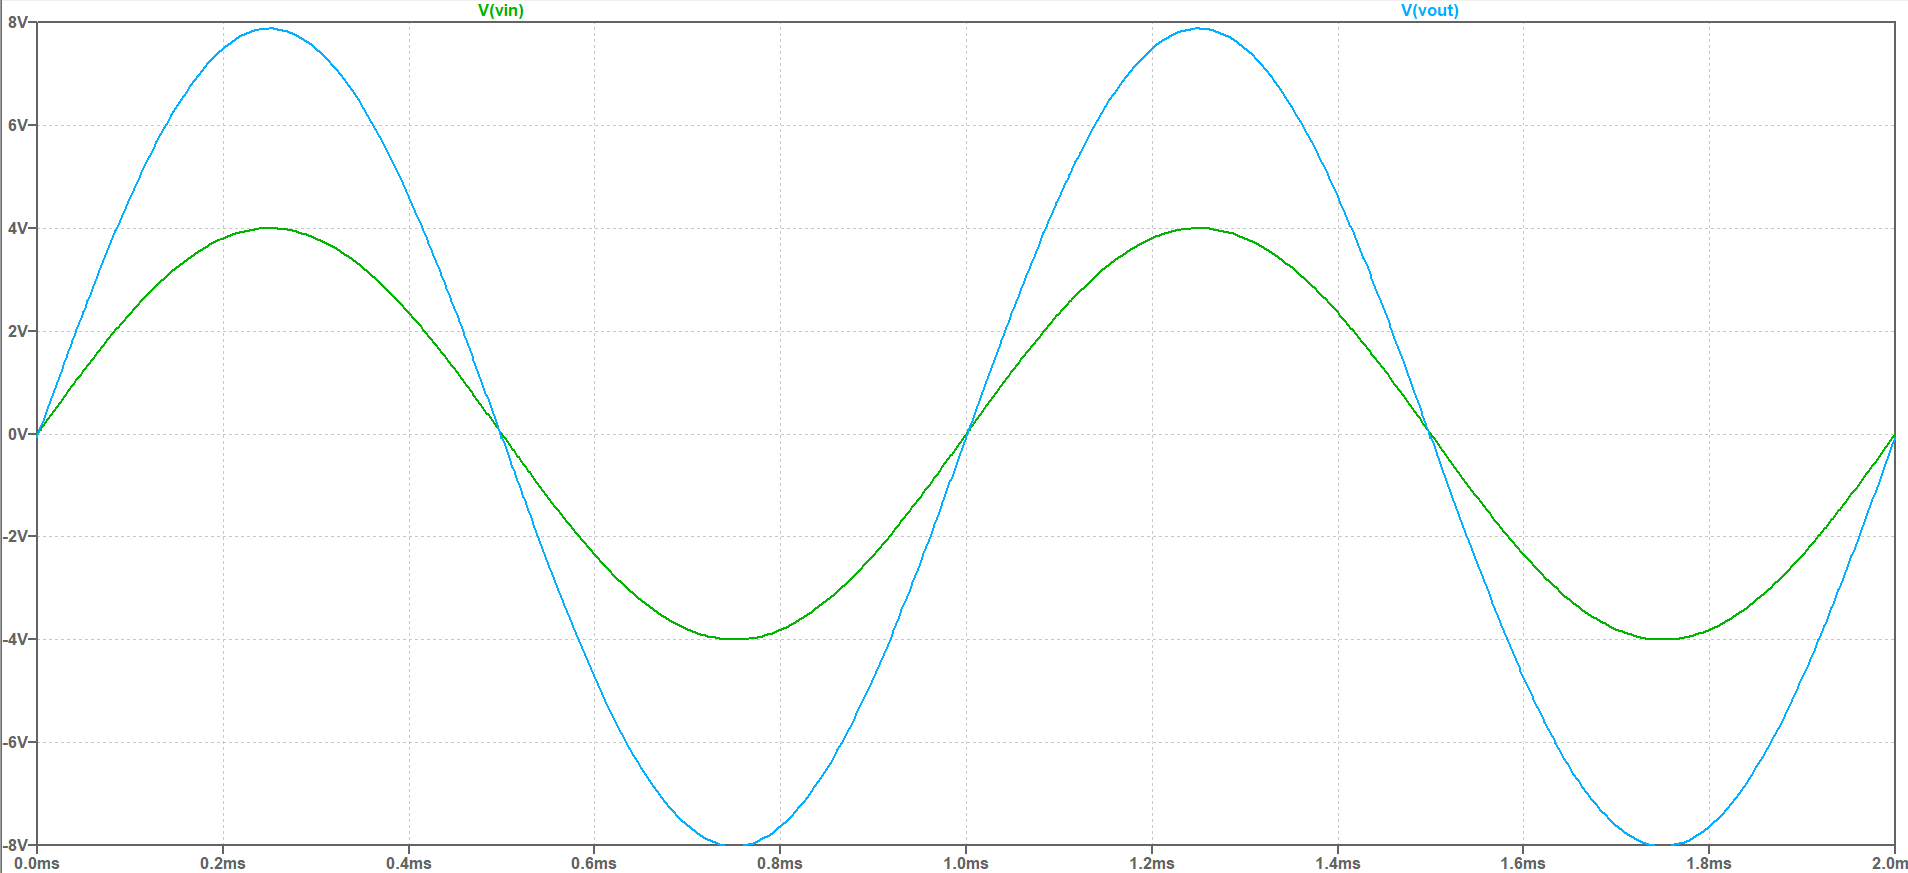
\includegraphics[scale=0.45]{Fig/gain.png}
        \label{fig:gain}
        \caption{the input and output of the circuit near maximum swing}
    \end{center}
\end{figure}

\textbf{II. Swing}\\
As seen below the swing is about 8.4V or 16.8V peak to peak: \\
\begin{figure}[H]
    \begin{center}
        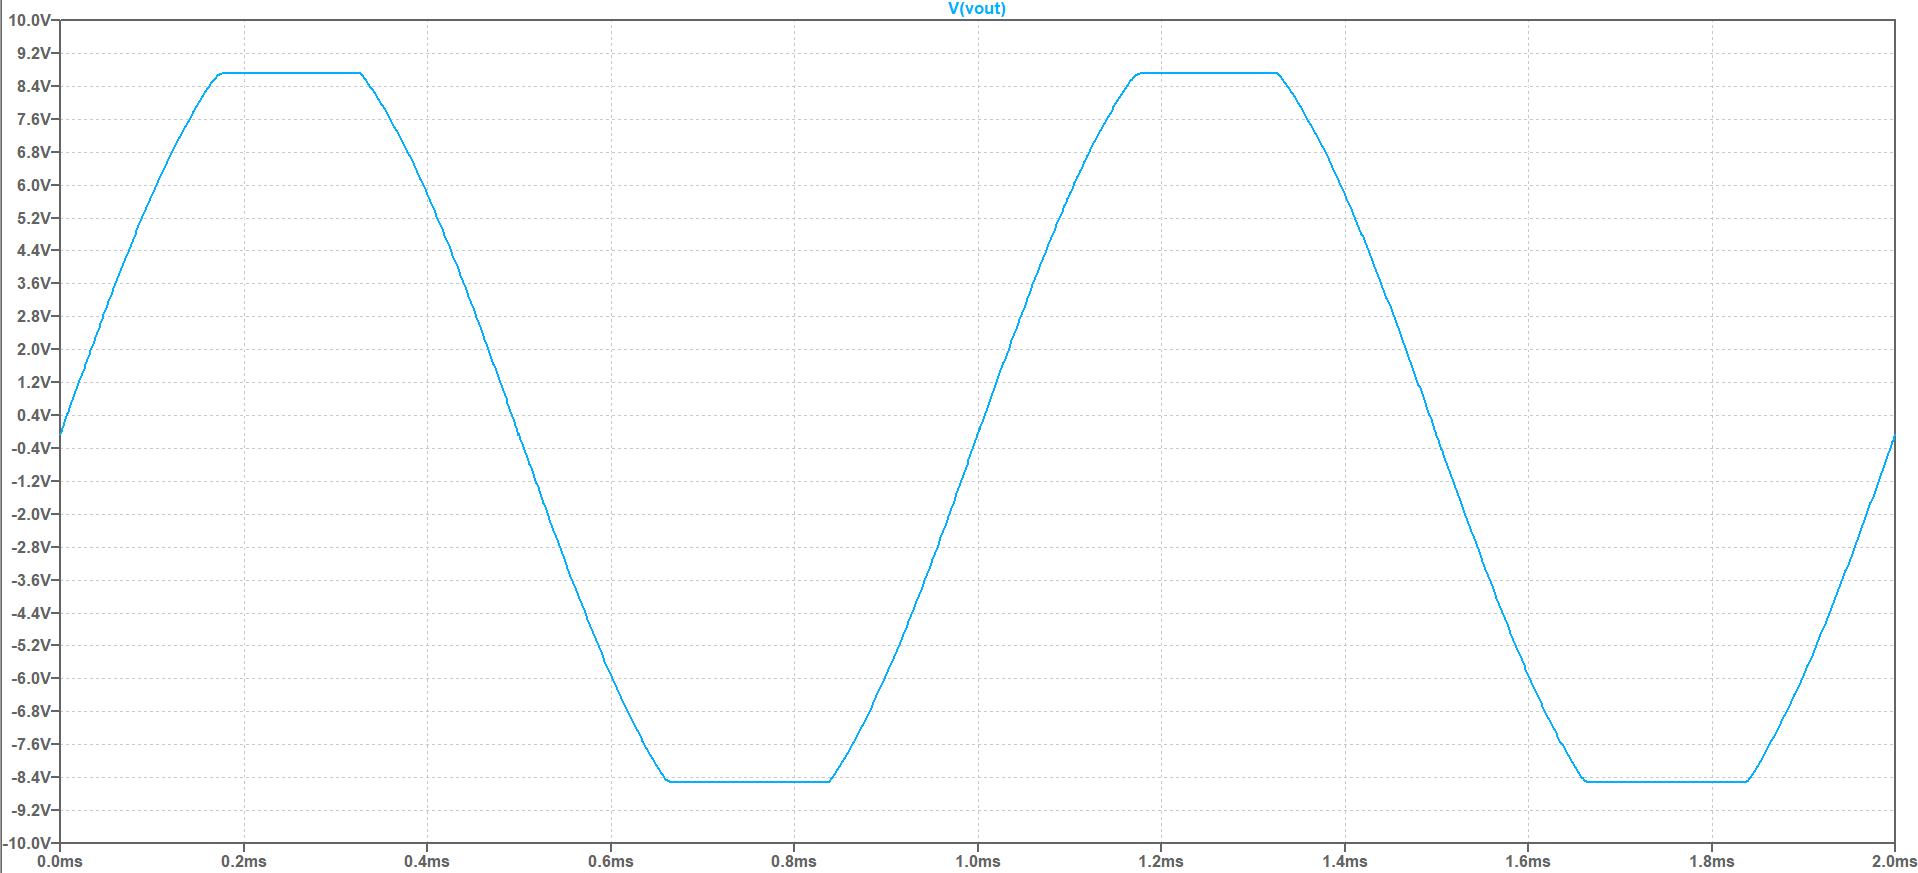
\includegraphics[scale=0.45]{Fig/swing.png}
        \label{fig:swing}
        \caption{the circuit output in its maximum swing bounds}
    \end{center}
\end{figure}

\textbf{III. Power}\\
As seen below the power given by sources about 49mW: \\
\begin{figure}[H]
    \begin{center}
        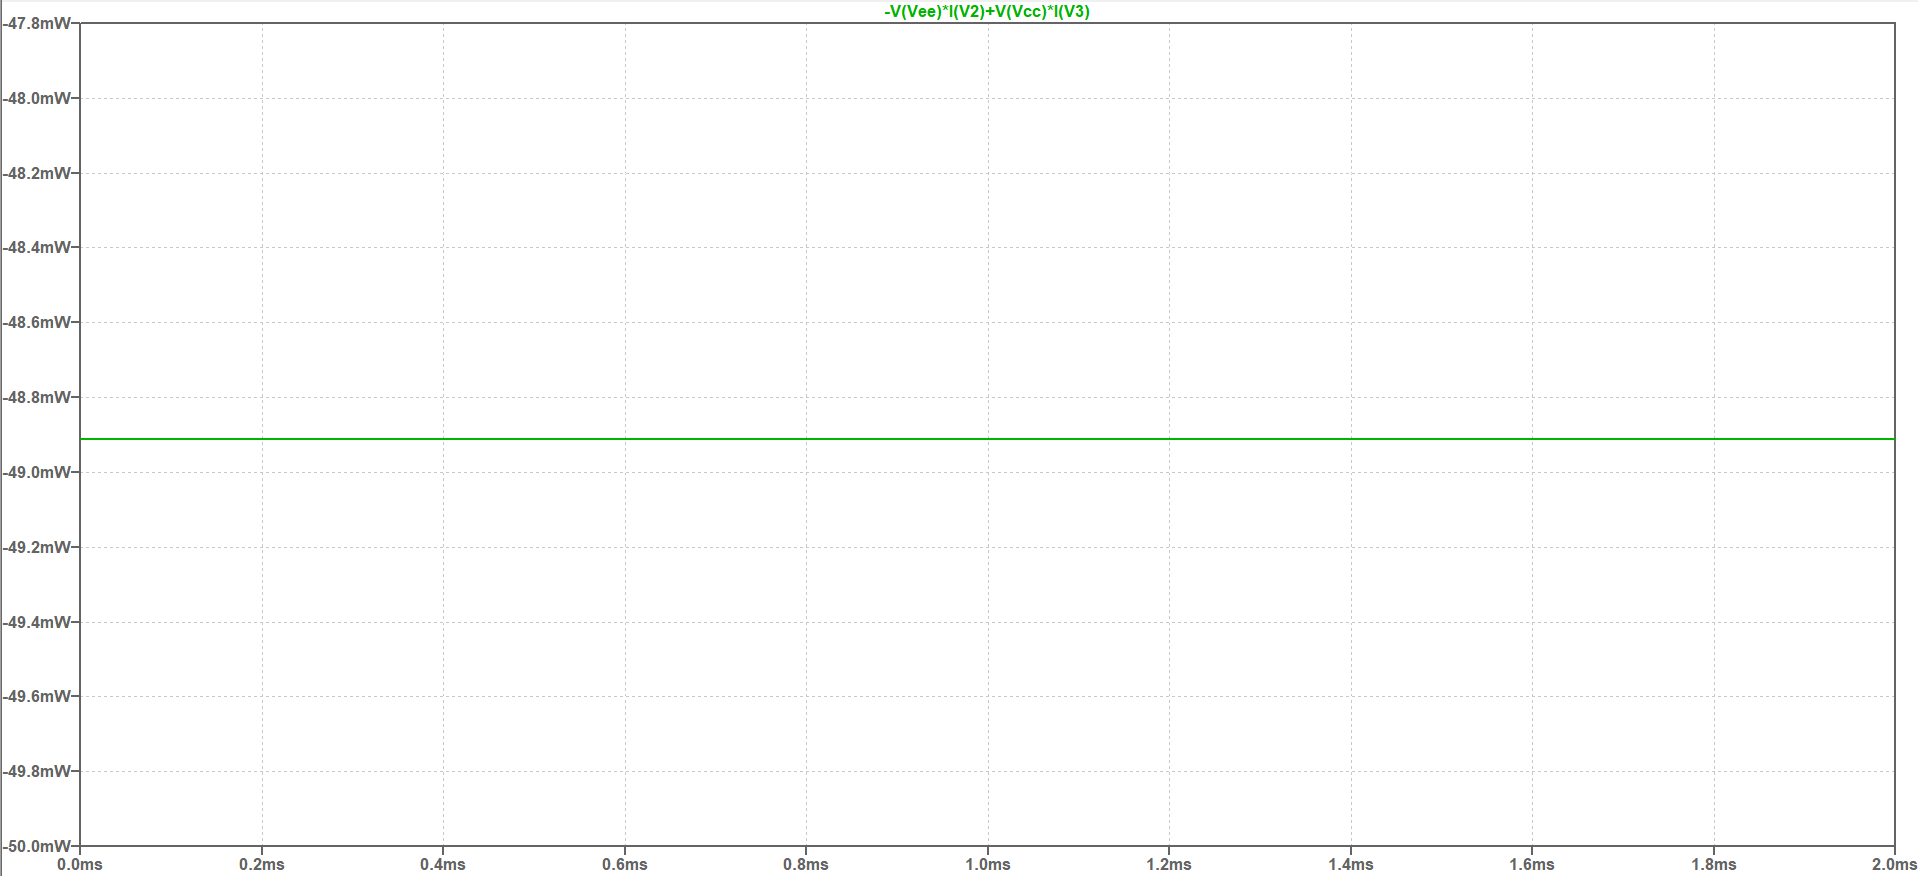
\includegraphics[scale=0.45]{Fig/power.png}
        \label{fig:power}
        \caption{the circuit power in 0 input}
    \end{center}
\end{figure}

\textbf{IV. THD}\\
As seen below the THD is about 0.026\%: \\
\begin{figure}[H]
    \begin{center}
        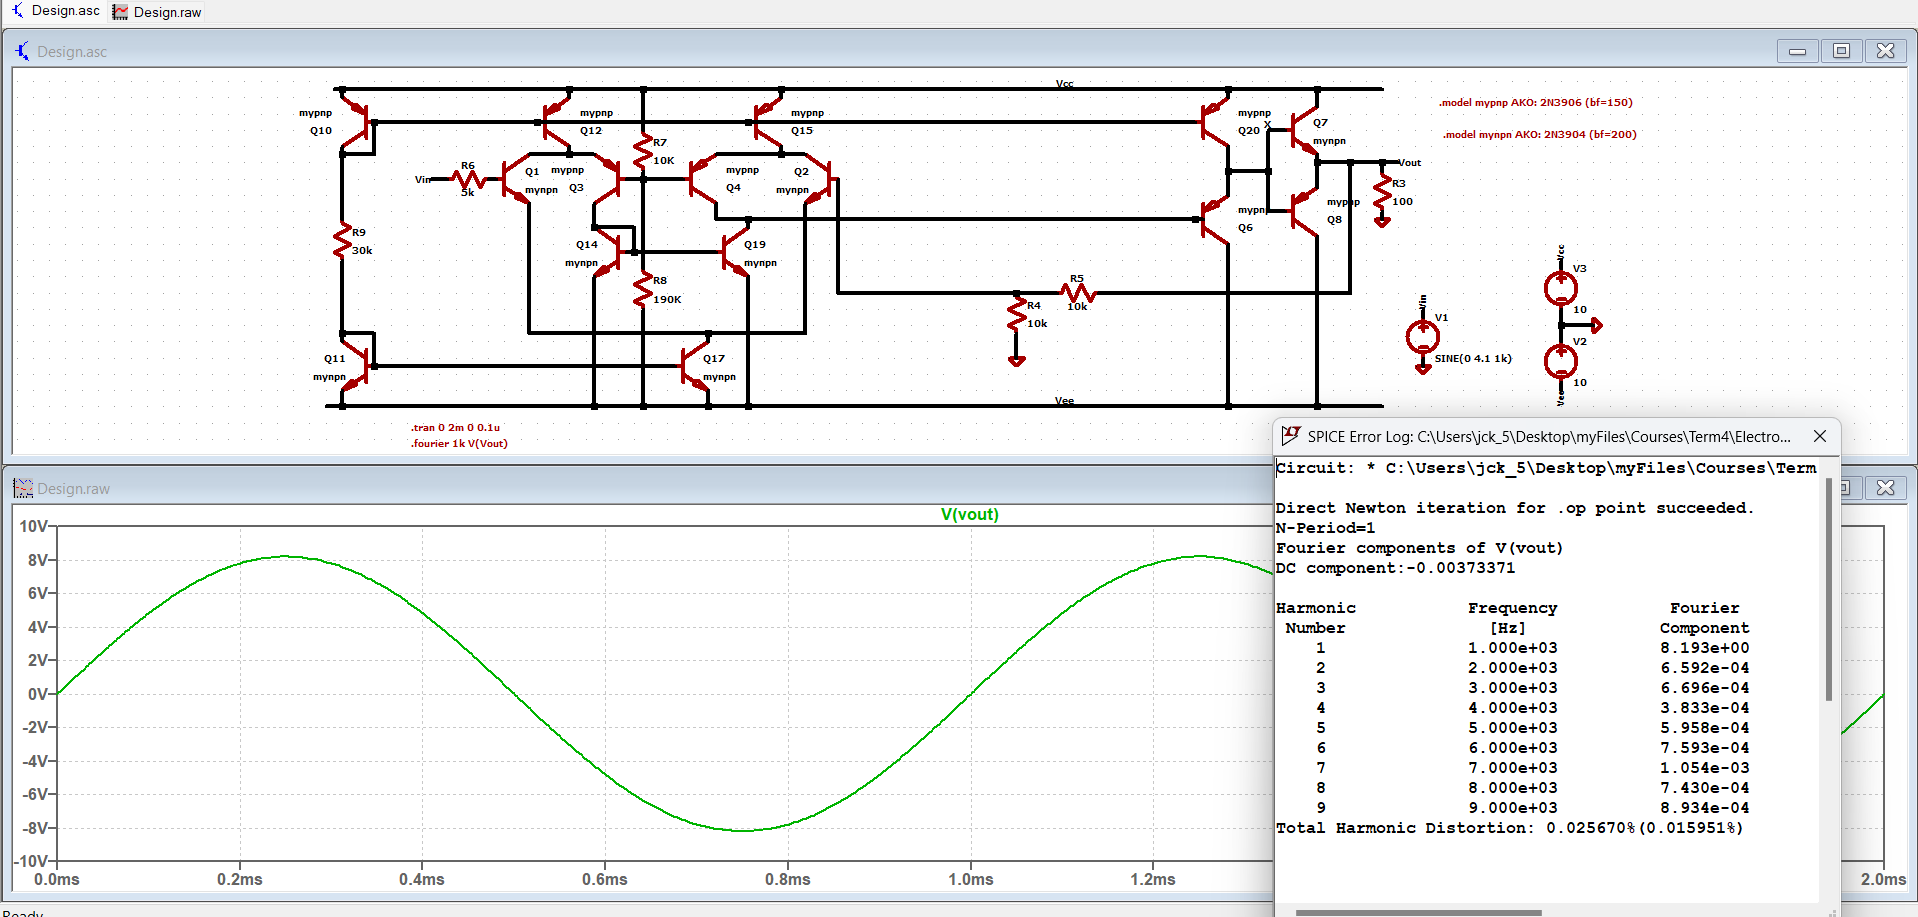
\includegraphics[scale=0.45]{Fig/THD.png}
        \label{fig:THD}
        \caption{the THD of the circuit power in 16.4V peak to peak}
    \end{center}
\end{figure}

\textbf{V. changing feedback resistors}\\
As seen below the THD increases by changing the feedback resistors to 50k
from 0.026\% to 0.033\%: \\
\begin{figure}[H]
    \begin{center}
        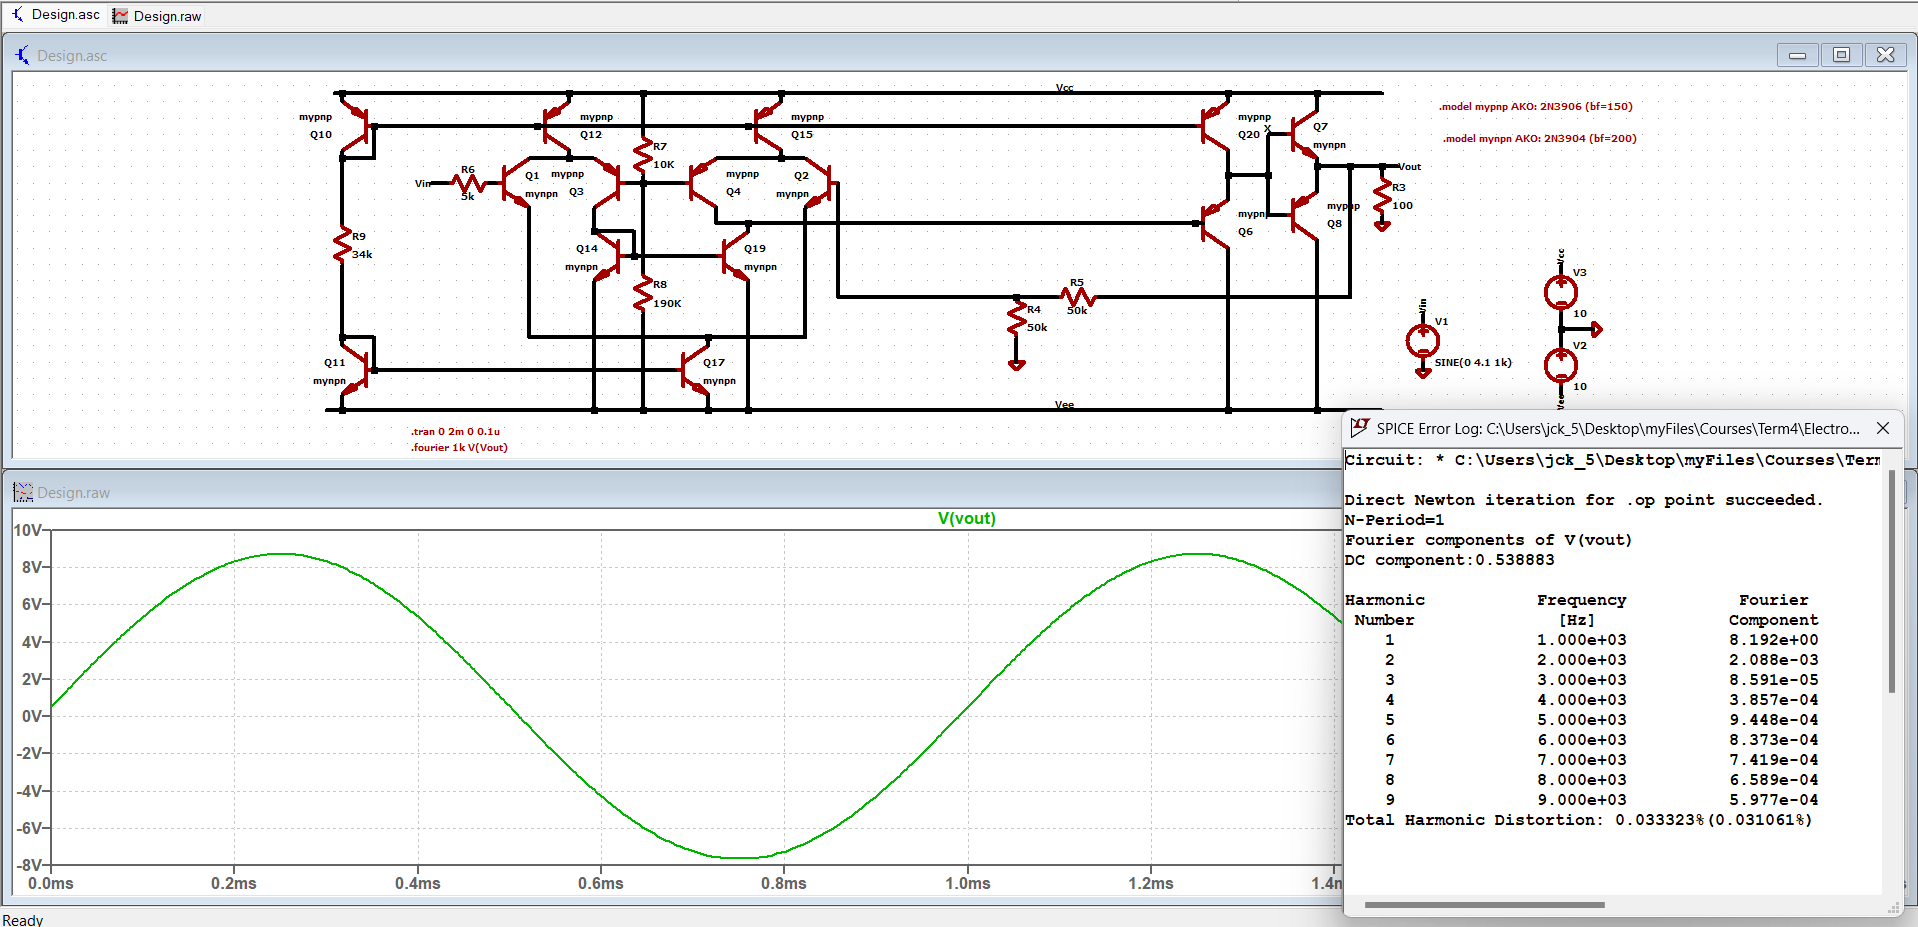
\includegraphics[scale=0.45]{Fig/50kdistortion.png}
        \label{fig:distortion50k}
        \caption{the THD with 50k feedback resistors}
    \end{center}
\end{figure}

\textbf{VI. explaining the reason 50k feedback resistor creates Distrotion} \\
because with 10k resistors the open loop resistance seen from Q1 and Q2 were the same
the differential stage was very symmetrical. by changing to 50k the base resistance of
Q2 is now 25k instead of 5k, this makes the differential stage a little bit asymmetric
and creates a little amount of distortion.\\


\end{document}
